\documentclass[11pt]{jsarticle}

\usepackage{SPR}

\headerSPR
\begin{document}
	\titleSPR{\number\year}{\number\month}{\number\day}{D2}{吉田 皓太郎}
%%%%%%%%%%%%%%%%%%%%%%%%%%%%%%%%%%%%%%
	\articleSPRabst
		\begin{itemize}
			\item 機械学習を用いたカップ形状の設計支援
			\item 着後形状予測のためのカップの変形解析
		\end{itemize}
		
		
	\articleSPRobj
		\begin{enumerate}
			\item 定性的な機能要求を満たせるようなカップ形状を設計できる
			\item 布の物性とカップのパターンがどのような結びつきを持っているかを調べることができる.
		\end{enumerate}
%%%%%%%%%%%%%%%%%%%%%%%%%%%%%%%%%%%%%%
% 1.前回からのノルマ
	\articleSPRitemsone
		%\begin{enumerate}
		%	\item A
		%\end{enumerate}
		
		\tableofcontents
		
		
%%%%%%%%%%%%%%%%%%%%%%%%%%%%%%%%%%%%%%
%\begin{itemize}
%	\item 新規手法について
%	\item ISFAアウトライン
%\end{itemize}
%%%%%%%%%%%%%%%%%%%%%%%%%%%%%%%%%%%%%%
% 2.具体的な成果
	\articleSPRitemstwo
	\renewcommand{\labelitemi}{$\blacktriangledown$}
	%\renewcommand{\labelitemi}{$\bigcirc$}
	\newcommand{\argmax}{\mathop{\rm arg~max}\limits}
	\newcommand{\argmin}{\mathop{\rm arg~min}\limits}
	\newcommand{\Ker}{{\rm Ker}}
	\newcommand{\rank}{{\rm rank}}
%%%%%%%%%%%%%%%%%%%%%%%%%%%%%%%%%%%%%
	\section{研究進捗について}
		\subsection{研究会進捗}
			$ \bd{y} = \bd{K}\bd{a} $とおき,$ \bd{a}^T \bd{K} \bd{a} / \lambda_{\min} - 1 $を制約を置く.これにより,桁数の小さい誤差も対応できるようにしている.(ここらへんは誤差評価の仕方に工夫のし甲斐があるかもしれない)
			また,局所解に陥らないように,目的関数に以下のような値を加えた.今回の$ \lambda $は,0.1に設定している.
			\begin{equation}
				\lambda \int_{0}^{L} \frac{1}{(\kappa - |\omega_{\eta}|)^2} ds
			\end{equation}
			
			計算結果を示す.制約に関しては二次形式に関する制約がだいたい数$ \% $程度の誤差にはなったところを終了判定の基準定めた.
			形状の比較をすると,zy平面からの形状はとても近しいが,zx平面で確認する図では,似てはいるが少し異なった形を出力した.
			
			しかし,対応する出力値$ \phi_1 \frac{V}{S} $を比較すると,だいたい相対誤差は2$ \% $ほどとなった.このラインは非常によいとまでは行かないが,ある程度はよい復元を得られたのではないかと考えられる.
			
			
			得られた結果とパラメータ元の形状比較
			\begin{figure}
				\begin{minipage}{0.5\hsize}
					\centering
					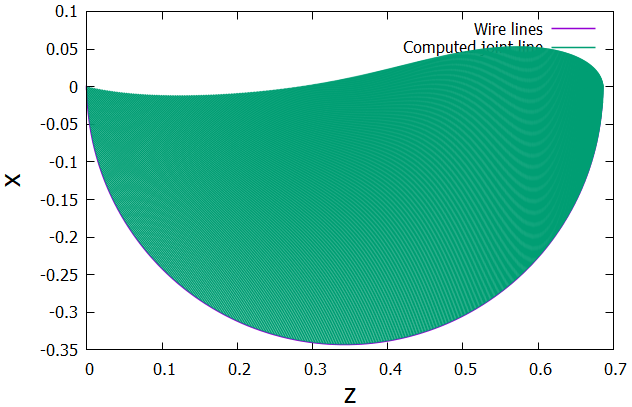
\includegraphics[width = \columnwidth]{./figure/ObtainedRidgeLinefromz-x.png}
				\end{minipage}
				\begin{minipage}{0.5\hsize}
					\centering
					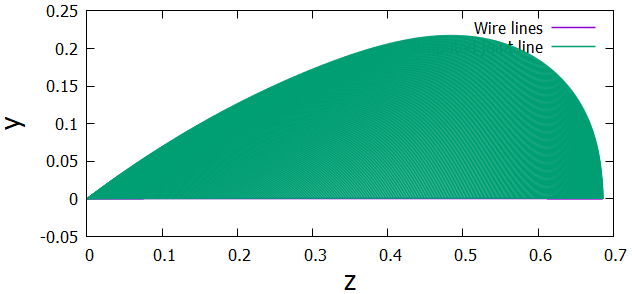
\includegraphics[width = \columnwidth]{./figure/ObtainedRidgeLinefromz-y.png}
				\end{minipage}
				\caption{元データ}
			\end{figure}
			\begin{figure}
				\begin{minipage}{0.5\hsize}
					\centering
					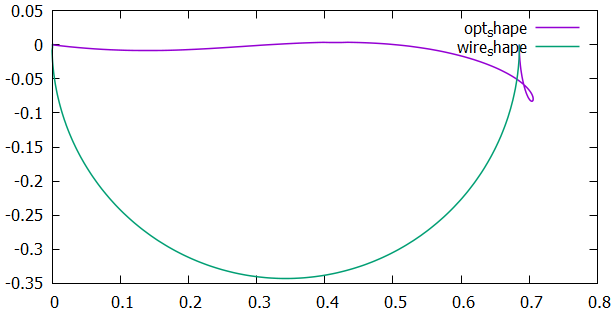
\includegraphics[width = \columnwidth]{./figure/AlignWire_xyview.png}
				\end{minipage}
				\begin{minipage}{0.5\hsize}
					\centering
					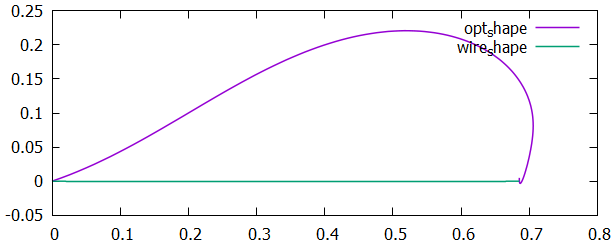
\includegraphics[width = \columnwidth]{./figure/AlignWire_xzview.png}
				\end{minipage}
			\caption{得られた形状}
			\end{figure}
		
		\subsection{ISCIEネタ再投稿の件について}
			日本語論文には,ISCIEに出すんですか?それとも,機械学会などの論文でしょうか?
			
			また,今回の論筋的に,ブラジャーの設計に強く押しすぎている点などもちょっとあったかなという気はしました.実世界へのアプリケーションを強く意識されてしまうのは,少し苦しいものもあり,D論の論筋的にも可展面の設計ができるという部分の論調も必要ではないかと思いました.そういった意味で,特に緒言の部分も再考し,タイトルも含めて考えるべきかと結果を踏まえ感じました.
			
			あとは,全体的に時間がぎりぎりだったのもあり,本文・回答書ともに全体的に雑さが目立ってしまいました.申し訳ないです.
			
			個人的には,英語論文に再チャレンジしたい気もします..時間的に厳しいかと思いますが.
	\section{To Do List}
		\begin{itemize}
			\item 投稿論文修正・文章再考
			\item 投稿論文のためのスクリプト作成し,追加数値実験を行う
		\end{itemize}
				
	\newpage
\vspace{10cm}
%%%%%%%%%%%%%%%%%%%%%%%%%%%%%%%%%%%%%%
% 3.達成できなかったこととその問題点
	%\articleSPRthree
	
%%%%%%%%%%%%%%%%%%%%%%%%%%%%%%%%%%%%%%

\vspace{14cm}
%%%%%%%%%%%%%%%%%%%%%%%%%%%%%%%%%%%%%%
	\articleSPRfour
	\articleSPRfive
\end{document}
